%%%%%%%%%%%%%%%%%%%%%%%%%%%%%%%%%%%%%%%%%%%%%%%%%%%%%%%%%%%%%%%%%%%%%%%%%%%%%%%%%%%%%
%%%%%%%%%%%%%%%%%%%%%%%%%%%%%%%%%%%%%%%%%%%%%%%%%%%%%%%%%%%%%%%%%%%%%%%%%%%%%%%%%%%%%

\setbeamercolor{block title}{bg=white, fg=black}
\setbeamercolor{block body}{bg=blue!20}

\begin{frame}
	\frametitle{Static analysis}

	\begin{block}{}
	\centering
	Static program analysis is the analysis of computer software which is performed without actually executing programs
	\end{block}
		
	\begin{figure}
	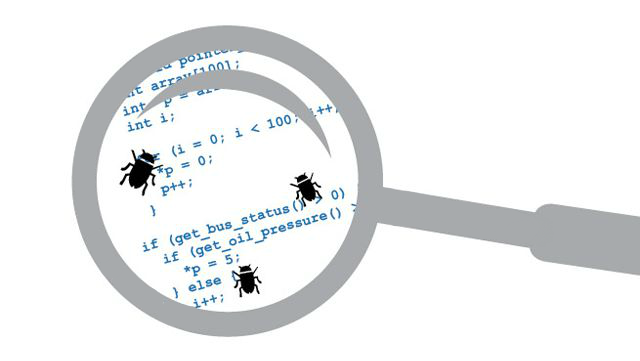
\includegraphics[width=70mm]{image/staticAnalysis}
	\end{figure}	
	
\end{frame}

%%%%%%%%%%%%%%%%%%%%%%%%%%%%%%%%%%%%%%%%%%%%%%%%%%%%%%%%%%%%%%%%%%%%%%%%%%%%%%%%%%%%%
%%%%%%%%%%%%%%%%%%%%%%%%%%%%%%%%%%%%%%%%%%%%%%%%%%%%%%%%%%%%%%%%%%%%%%%%%%%%%%%%%%%%%


\begin{frame}
	\frametitle{Performance problem}

	\begin{block}{}
		\centering
			Most static analyses are pretty limited in their ability to scale to large industrial software and our bounded model checking tool Borealis is not exception 
	\end{block}

	\begin{block}{}
		\centering
		We decided to try an approach of \textit{scaling} Borealis to multiple cores
	\end{block}
\end{frame}

%%%%%%%%%%%%%%%%%%%%%%%%%%%%%%%%%%%%%%%%%%%%%%%%%%%%%%%%%%%%%%%%%%%%%%%%%%%%%%%%%%%%%
%%%%%%%%%%%%%%%%%%%%%%%%%%%%%%%%%%%%%%%%%%%%%%%%%%%%%%%%%%%%%%%%%%%%%%%%%%%%%%%%%%%%%

\setbeamercolor{block title}{bg=white, fg=black}
\setbeamercolor{block body}{bg=blue!20}

\begin{frame}
	\frametitle{Bounded model checking}
	
	\begin{block}{}
	\centering
	Model checking is the algorithmic analysis of programs to prove properties
of their executions
	\end{block}
		
	\begin{block}{}
	\centering
	Bounded model checking is extension of model checking, which solves the problem of combinatorial explosion of state space by bounding the infinite branches of program
	\end{block}
		
\end{frame}

%%%%%%%%%%%%%%%%%%%%%%%%%%%%%%%%%%%%%%%%%%%%%%%%%%%%%%%%%%%%%%%%%%%%%%%%%%%%%%%%%%%%%
%%%%%%%%%%%%%%%%%%%%%%%%%%%%%%%%%%%%%%%%%%%%%%%%%%%%%%%%%%%%%%%%%%%%%%%%%%%%%%%%%%%%%

\setbeamercolor{block title}{bg=white, fg=black}
\setbeamercolor{block body}{bg=blue!20}

\begin{frame}[fragile]
	\frametitle{Satisfiability modulo theories}
	
	\textbf{SAT problem}:
	\begin{lstlisting}[style=crs_cpp, basicstyle = {\ttfamily \scriptsize},]
bool a, b, c, d
check-sat:
a & !a & b & c & d
	\end{lstlisting}
	
	\textbf{SMT problem}:
	\begin{lstlisting}[style=crs_cpp, basicstyle = {\ttfamily \scriptsize},]
int x, y
bool a
check-sat:
(x + y < 0) & (x = 0) & !(y + 1 = 0)
	\end{lstlisting}
			
\end{frame}


%%%%%%%%%%%%%%%%%%%%%%%%%%%%%%%%%%%%%%%%%%%%%%%%%%%%%%%%%%%%%%%%%%%%%%%%%%%%%%%%%%%%%
%%%%%%%%%%%%%%%%%%%%%%%%%%%%%%%%%%%%%%%%%%%%%%%%%%%%%%%%%%%%%%%%%%%%%%%%%%%%%%%%%%%%%

\begin{frame}
	\frametitle{Borealis}
	
	\begin{figure}
	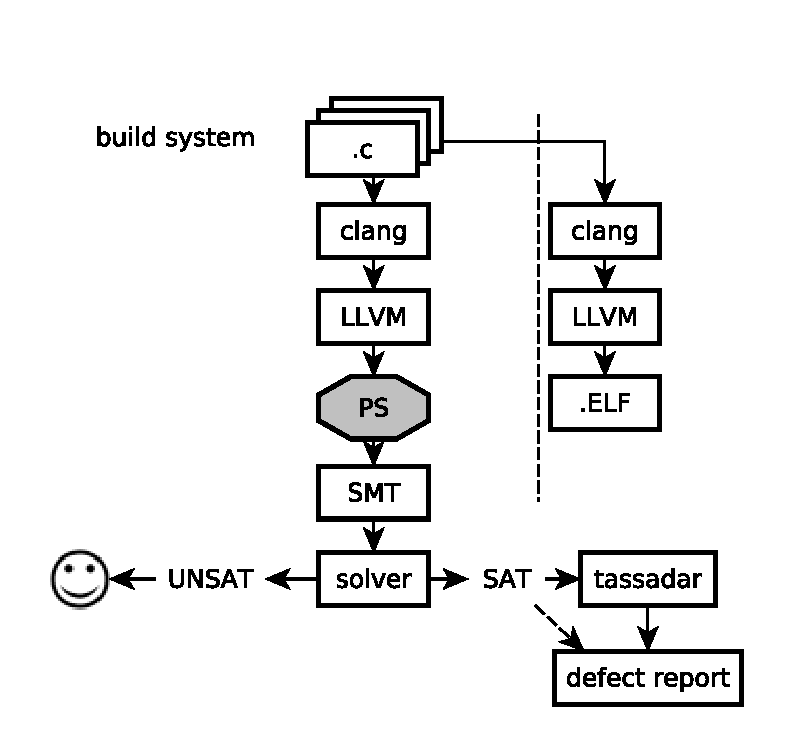
\includegraphics[width=80mm]{image/BorealisOverview}
	\end{figure}	
	
\end{frame}

%%%%%%%%%%%%%%%%%%%%%%%%%%%%%%%%%%%%%%%%%%%%%%%%%%%%%%%%%%%%%%%%%%%%%%%%%%%%%%%%%%%%%
%%%%%%%%%%%%%%%%%%%%%%%%%%%%%%%%%%%%%%%%%%%%%%%%%%%%%%%%%%%%%%%%%%%%%%%%%%%%%%%%%%%%%

\setbeamercolor{block title}{bg=white, fg=black}
\setbeamercolor{block body}{bg=blue!20}

\begin{frame}[fragile]
	\frametitle{Predicate state}
	
	\begin{block}{}
	Predicate state is a simplified representation of the original program
	\end{block}
	
	\begin{columns}
	\column{0.5\textwidth}
	\begin{lstlisting}[language=PS, frame=single]
(
  %0=alloca(1,(1 * 1)),
  %1=alloca(1,(1 * 1)),
  %2=*(%0),
  cmp=(%2 > 0)
)->(BEGIN
<OR>(
  @P cmp=true,
  %3=*(%0),
  add=(2 - %3),
  *%1=add,
),
<OR>(
  @P cmp=false
)
END)->(
  \result_foo=0
)
	\end{lstlisting}
	
	\end{columns}
	
\end{frame}

%%%%%%%%%%%%%%%%%%%%%%%%%%%%%%%%%%%%%%%%%%%%%%%%%%%%%%%%%%%%%%%%%%%%%%%%%%%%%%%%%%%%%
%%%%%%%%%%%%%%%%%%%%%%%%%%%%%%%%%%%%%%%%%%%%%%%%%%%%%%%%%%%%%%%%%%%%%%%%%%%%%%%%%%%%%

\begin{frame}
	\frametitle{Program representation}
	\begin{figure}
	\includegraphics[width=110mm, keepaspectratio]{image/PSDef}
	\end{figure}
\end{frame}

%%%%%%%%%%%%%%%%%%%%%%%%%%%%%%%%%%%%%%%%%%%%%%%%%%%%%%%%%%%%%%%%%%%%%%%%%%%%%%%%%%%%%
%%%%%%%%%%%%%%%%%%%%%%%%%%%%%%%%%%%%%%%%%%%%%%%%%%%%%%%%%%%%%%%%%%%%%%%%%%%%%%%%%%%%%

\begin{frame}
	\frametitle{SMT formulae}
\begin{itemize}
	\item The resulting SMT formulae need to be checked for correctness
	\item Borealis asks $B \ \wedge \ !Q$ is satisfiable
	\item If unsatisfiable, $B \ \wedge \ Q$ and the program is correct
	\item If satisfiable, the program contains a bug
	\item Process is repeated for every program point which might trigger an error
\end{itemize}
\end{frame}

%%%%%%%%%%%%%%%%%%%%%%%%%%%%%%%%%%%%%%%%%%%%%%%%%%%%%%%%%%%%%%%%%%%%%%%%%%%%%%%%%%%%%
%%%%%%%%%%%%%%%%%%%%%%%%%%%%%%%%%%%%%%%%%%%%%%%%%%%%%%%%%%%%%%%%%%%%%%%%%%%%%%%%%%%%%

\setbeamercolor{block title}{bg=white, fg=black}
\setbeamercolor{block body}{bg=red!20}
\begin{frame}
\frametitle{Problem}
\begin{block}{}
	\centering
	The sheer number of SMT queries involved in checking a large program is enough to take a huge processing time
\end{block}

\setbeamercolor{block title}{bg=white, fg=black}
\setbeamercolor{block body}{bg=blue!20}

\begin{block}{}
	\centering
	We decided to try and scale Borealis to multiple cores on our RSC Tornado supercomputer cluster
\end{block}
\end{frame}

%%%%%%%%%%%%%%%%%%%%%%%%%%%%%%%%%%%%%%%%%%%%%%%%%%%%%%%%%%%%%%%%%%%%%%%%%%%%%%%%%%%%%
%%%%%%%%%%%%%%%%%%%%%%%%%%%%%%%%%%%%%%%%%%%%%%%%%%%%%%%%%%%%%%%%%%%%%%%%%%%%%%%%%%%%%

\begin{frame}
\frametitle{RSC Tornado supercomputer}
\begin{itemize}
\item 712 dual-processor nodes with 1424 Intel Xeon E5-2697
\item Each node has 64 GB of DDR4 RAM and local 120 GB SSD storage
\item Shared 1 PB Lustre storage
\item 612 nodes
\end{itemize}
\end{frame}
